\documentclass[letta4 paper]{article}
% Set target color model to RGB
\usepackage[inner=2.0cm,outer=2.0cm,top=2.5cm,bottom=2.5cm]{geometry}
\usepackage{setspace}
\usepackage[rgb]{xcolor}
\usepackage{verbatim}
\usepackage{subcaption}
\usepackage{amsgen,amsmath,amstext,amsbsy,amsopn,tikz,amssymb,tkz-linknodes}
\usepackage{fancyhdr}
\usepackage[colorlinks=true, urlcolor=blue,  linkcolor=blue, citecolor=blue]{hyperref}
\usepackage[colorinlistoftodos]{todonotes}
\usepackage{rotating}
\usepackage{listings}
\usepackage{algorithm}
\usepackage{algorithmic}
\usepackage{ulem}
\usepackage{pdflscape}
\usepackage{changepage}
\lstset{
%	language=bash,
	basicstyle=\ttfamily
}

\newcommand{\ra}[1]{\renewcommand{\arraystretch}{#1}}

\newtheorem{thm}{Theorem}[section]
\newtheorem{prop}[thm]{Proposition}
\newtheorem{lem}[thm]{Lemma}
\newtheorem{cor}[thm]{Corollary}
\newtheorem{defn}[thm]{Definition}
\newtheorem{rem}[thm]{Remark}
\numberwithin{equation}{section}
\graphicspath{ {./img/} }

\newcommand{\homework}[6]{
   \pagestyle{myheadings}
   \thispagestyle{plain}
   \newpage
   \setcounter{page}{1}
   \noindent
   \begin{center}
   \framebox{
      \vbox{\vspace{2mm}
    \hbox to 6.28in { {\bf F1TENTH Autonomous Racing \hfill {\small (#2 26.05.2020)}} }
       \vspace{6mm}
       \hbox to 6.28in { {\Large \hfill #1  \hfill} }
       \vspace{6mm}
       \hbox to 6.28in { {\it Instructor: {\rm GROSU} \hfill Name: {\rm \textbf{TEAM 3} (Adelmann, Brantner, Lukitsch, Pintaric)} {}} }
       %\hbox to 6.28in { {\it T\textbf{A:} #4  \hfill #6}}
      \vspace{2mm}}
   }
   \end{center}
   \markboth{#5 -- #1}{#5 -- #1}
   \vspace*{4mm}
}


\newcommand{\problem}[3]{~\\\fbox{\textbf{Problem #1: #2}}\hfill (#3 points)\newline}
\newcommand{\subproblem}[1]{~\newline\textbf{(#1)}}
\newcommand{\D}{\mathcal{D}}
\newcommand{\Hy}{\mathcal{H}}
\newcommand{\VS}{\textrm{VS}}
\newcommand{\solution}{~\newline\textbf{\textit{(Solution)}} }

\newcommand{\bbF}{\mathbb{F}}
\newcommand{\bbX}{\mathbb{X}}
\newcommand{\bI}{\mathbf{I}}
\newcommand{\bX}{\mathbf{X}}
\newcommand{\bY}{\mathbf{Y}}
\newcommand{\bepsilon}{\boldsymbol{\epsilon}}
\newcommand{\balpha}{\boldsymbol{\alpha}}
\newcommand{\bbeta}{\boldsymbol{\beta}}
\newcommand{\0}{\mathbf{0}}


\usepackage{booktabs}



\begin{document}

	\homework {Lab 7: Motion Planning - Written Answers}{Due Date:}{INSTRUCTOR}{}{STUDENT NAME}{ID}
	\thispagestyle{empty}
	% -------- DO NOT REMOVE THIS LICENSE PARAGRAPH	----------------%
	\begin{table}[h]
		\begin{tabular}{l p{14cm}}
		\raisebox{-2cm}{
\includegraphics[scale=0.5, height=2.5cm]{f1_stickers_04} } & \textit{This lab and all related course material on \href{http://f1tenth.org/}{F1TENTH Autonomous Racing} has been developed by the Safe Autonomous Systems Lab at the University of Pennsylvania (Dr. Rahul Mangharam). It is licensed under a \href{https://creativecommons.org/licenses/by-nc-sa/4.0/}{Creative Commons Attribution-NonCommercial-ShareAlike 4.0 International License.} You may download, use, and modify the material, but must give attribution appropriately. Best practices can be found \href{https://wiki.creativecommons.org/wiki/best_practices_for_attribution}{here}.}
		\end{tabular}
	\end{table}
	% -------- DO NOT REMOVE THIS LICENSE PARAGRAPH	----------------%
	
	\noindent \large{\textbf{Course Policy:}} Read all the instructions below carefully before you start working on the assignment, and before you make a submission. All sources of material must be cited. The University Academic Code of Conduct will be strictly enforced.
	\\
	\\
	\textbf{THIS IS A GROUP ASSIGNMENT}. Submit one from each team.\\

	\section{Part A: Written assignment}
	\begin{figure}[!hb]
		\begin{center}
			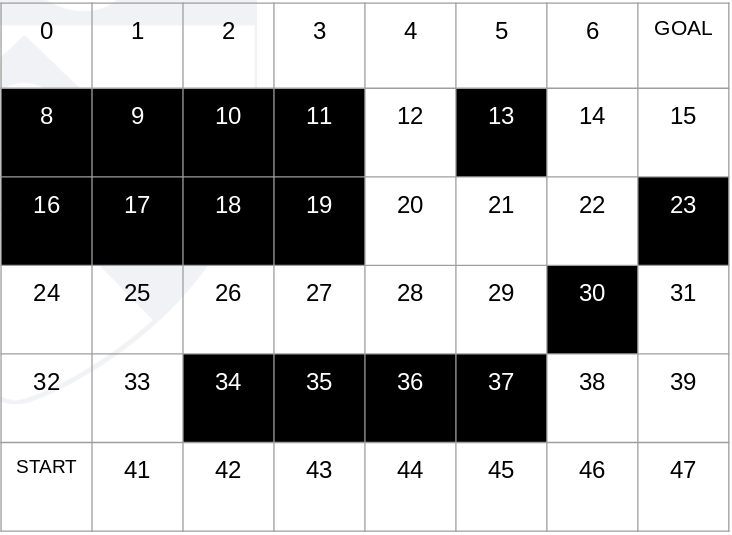
\includegraphics[scale=0.4]{grid_world.png}
		\end{center}
		\caption{Grid World}
		\label{fig:gridworld}
	\end{figure}
	\subsection{Grid world planning with Dijkstra's}
	Using figure \ref{fig:gridworld}, write out steps for Dijkstra's algorithm (\textbf{8-connected}, assume uniform cost for each action). At each step, list the grid cells in the open set with their running cost and the grid cells in the visited set. Write the final path found as a list of grid cell ids.\\
	\\
	\textbf{Solution:}\\
	
	On the following pages the calculation of the Dijkstra-Algorithm is shown. Our found path has a length of 7 and was found by always selecting the cell with the loweset index first, if there were 2 cells with the same cost.
	\\
	\\
	The found path is: $S \implies 33 \implies 26 \implies 27 \implies 20 \implies 21 \implies 14 \implies G$
	\\
	\\
	The set of the \texttt{visited} cells can be seen in the \texttt{Sel} column, for each step all the upwards entries of the column have been visited previously. Also the different sets with the currently \texttt{open} cells and their current costs can be seen in the vertical line of each step. If they have already been visited, the have no cost entry, if there has not been a path found the cost is listed with $\infty$ and the currently selected cell is listed in bold font, if it is selected and visited in the current step. \\
	In the last column \texttt{Pre} the previous cell of the selected cell is listed, so we can tranverse the found tree backwards from a certain goal-cell. The found path from Start to Goal is underlined in the \texttt{Pre} column. 
	
	%\begin{landscape}

\begin{table}
\centering
\begin{tabular}{l|ll}
Step & Open(Cost) & Visited  \\ 
\hline
0    & 41, 42, 43, 44, 45, 46, 47, 32, 33, 38, 39, 24, 25, 26, 27, 28, 29, 31, 20, 21, 22, 12, 14, 15, 0, 1, 2, 3, 4, 5, 6, G           & S        \\
1    & 41(1), 42, 43, 44, 45, 46, 47, 32(1), 33(1), 38, 39, 24, 25, 26, 27, 28, 29, 31, 20, 21, 22, 12, 14, 15, 0, 1, 2, 3, 4, 5, 6, G           & S, 32    \\
2    & 41(1), 42, 43, 44, 45, 46, 47, 32(1), 33(1), 38, 39, 24, 25, 26, 27, 28, 29, 31, 20, 21, 22, 12, 14, 15, 0, 1, 2, 3, 4, 5, 6, G           & S, 32 , 33        \\
3    &            & S, 32 , 33, 41         \\
4    &            & S, 32 , 33, 41, 24         \\
5    &            & S, 32 , 33, 41, 24, 25         \\
6    &            & S, 32 , 33, 41, 24, 25, 26         \\
7    &            & S, 32 , 33, 41, 24, 25, 26, 42         \\
8    &            & S, 32 , 33, 41, 24, 25, 26, 42, 27         \\
9    &            & S, 32 , 33, 41, 24, 25, 26, 42, 27, 43         \\
10   &            & S, 32 , 33, 41, 24, 25, 26, 42, 27, 43, 20          \\
11   &            & S, 32 , 33, 41, 24, 25, 26, 42, 27, 43, 20, 28         \\
12   &            & S, 32 , 33, 41, 24, 25, 26, 42, 27, 43, 20, 28, 44          \\
13   &            & S, 32 , 33, 41, 24, 25, 26, 42, 27, 43, 20, 28, 44, 12        \\
14   &            & S, 32 , 33, 41, 24, 25, 26, 42, 27, 43, 20, 28, 44, 12, 21         \\
15   &            &  S, 32 , 33, 41, 24, 25, 26, 42, 27, 43, 20, 28, 44, 12, 21, 29        \\
16   &            & S, 32 , 33, 41, 24, 25, 26, 42, 27, 43, 20, 28, 44, 12, 21, 29, 45         \\
17   &            & S, 32 , 33, 41, 24, 25, 26, 42, 27, 43, 20, 28, 44, 12, 21, 29, 45, 3         \\
18   &            &  S, 32 , 33, 41, 24, 25, 26, 42, 27, 43, 20, 28, 44, 12, 21, 29, 45, 3, 4         \\
19   &            & S, 32 , 33, 41, 24, 25, 26, 42, 27, 43, 20, 28, 44, 12, 21, 29, 45, 3, 4, 5          \\
20   &            &  S, 32 , 33, 41, 24, 25, 26, 42, 27, 43, 20, 28, 44, 12, 21, 29, 45, 3, 4, 5, 14        \\
21   &            & S, 32 , 33, 41, 24, 25, 26, 42, 27, 43, 20, 28, 44, 12, 21, 29, 45, 3, 4, 5, 14, 22           \\
22   &            & S, 32 , 33, 41, 24, 25, 26, 42, 27, 43, 20, 28, 44, 12, 21, 29, 45, 3, 4, 5, 14, 22, 33         \\
23   &            & S, 32 , 33, 41, 24, 25, 26, 42, 27, 43, 20, 28, 44, 12, 21, 29, 45, 3, 4, 5, 14, 22, 33, 46          \\
24   &            & S, 32 , 33, 41, 24, 25, 26, 42, 27, 43, 20, 28, 44, 12, 21, 29, 45, 3, 4, 5, 14, 22, 33, 46, 2         \\
25   &            & S, 32 , 33, 41, 24, 25, 26, 42, 27, 43, 20, 28, 44, 12, 21, 29, 45, 3, 4, 5, 14, 22, 33, 46, 2, 6         \\
26   &            & S, 32 , 33, 41, 24, 25, 26, 42, 27, 43, 20, 28, 44, 12, 21, 29, 45, 3, 4, 5, 14, 22, 33, 46, 2, 6, 15          \\
27   &            & S, 32 , 33, 41, 24, 25, 26, 42, 27, 43, 20, 28, 44, 12, 21, 29, 45, 3, 4, 5, 14, 22, 33, 46, 2, 6, 15, 31         \\
28   &            &  S, 32 , 33, 41, 24, 25, 26, 42, 27, 43, 20, 28, 44, 12, 21, 29, 45, 3, 4, 5, 14, 22, 33, 46, 2, 6, 15, 31, 39        \\
29   &            &  S, 32 , 33, 41, 24, 25, 26, 42, 27, 43, 20, 28, 44, 12, 21, 29, 45, 3, 4, 5, 14, 22, 33, 46, 2, 6, 15, 31, 39, 47        \\
30   &            &  S, 32 , 33, 41, 24, 25, 26, 42, 27, 43, 20, 28, 44, 12, 21, 29, 45, 3, 4, 5, 14, 22, 33, 46, 2, 6, 15, 31, 39, 47, G        \\
31   &            & S, 32 , 33, 41, 24, 25, 26, 42, 27, 43, 20, 28, 44, 12, 21, 29, 45, 3, 4, 5, 14, 22, 33, 46, 2, 6, 15, 31, 39, 47, G, 1        \\
32   &            & S, 32 , 33, 41, 24, 25, 26, 42, 27, 43, 20, 28, 44, 12, 21, 29, 45, 3, 4, 5, 14, 22, 33, 46, 2, 6, 15, 31, 39, 47, G, 1, 0        
\end{tabular}
\end{table}

\end{landscape}
	% \usepackage{color}
% \usepackage[normalem]{ulem}
\begin{landscape}
\thispagestyle{empty}
\begin{table}
	\centering
	\begin{adjustwidth}{-2.6cm}{}
		\resizebox{\paperheight}{!}{
	\begin{tabular}{l|lllllllllllllllllllllllllllllllll|ll}
		Step & S          & 41                                                              & 42                                                              & 43                                                              & 44                                                              & 45                                                              & 46                                                              & 47                                                              & 32                                                              & 33                                                              & 38                                                              & 39                                                              & 24                                                              & 25                                                              & 26                                                              & 27                                                              & 28                                                              & 29                                                              & 31                                                              & 20                                                              & 21                                                              & 22                                                              & 12                                                              & 14                                                              & 15                                                              & 0                                                               & 1                                                               & 2                                                               & 3                                                               & 4                                                               & 5                                                               & 6                                                               & G                                                               & Sel        & Prev        \\ 
		\hline
		0    & \textbf{0} & $\textcolor[rgb]{0.541,0.29,0.043}{\infty}$ & $\textcolor[rgb]{0.541,0.29,0.043}{\infty}$ & $\textcolor[rgb]{0.541,0.29,0.043}{\infty}$ & $\textcolor[rgb]{0.541,0.29,0.043}{\infty}$ & $\textcolor[rgb]{0.541,0.29,0.043}{\infty}$ & $\textcolor[rgb]{0.541,0.29,0.043}{\infty}$ & $\textcolor[rgb]{0.541,0.29,0.043}{\infty}$ & $\textcolor[rgb]{0.541,0.29,0.043}{\infty}$ & $\textcolor[rgb]{0.541,0.29,0.043}{\infty}$ & $\textcolor[rgb]{0.541,0.29,0.043}{\infty}$ & $\textcolor[rgb]{0.541,0.29,0.043}{\infty}$ & $\textcolor[rgb]{0.541,0.29,0.043}{\infty}$ & $\textcolor[rgb]{0.541,0.29,0.043}{\infty}$ & $\textcolor[rgb]{0.541,0.29,0.043}{\infty}$ & $\textcolor[rgb]{0.541,0.29,0.043}{\infty}$ & $\textcolor[rgb]{0.541,0.29,0.043}{\infty}$ & $\textcolor[rgb]{0.541,0.29,0.043}{\infty}$ & $\textcolor[rgb]{0.541,0.29,0.043}{\infty}$ & $\textcolor[rgb]{0.541,0.29,0.043}{\infty}$ & $\textcolor[rgb]{0.541,0.29,0.043}{\infty}$ & $\textcolor[rgb]{0.541,0.29,0.043}{\infty}$ & $\textcolor[rgb]{0.541,0.29,0.043}{\infty}$ & $\textcolor[rgb]{0.541,0.29,0.043}{\infty}$ & $\textcolor[rgb]{0.541,0.29,0.043}{\infty}$ & $\textcolor[rgb]{0.541,0.29,0.043}{\infty}$ & $\textcolor[rgb]{0.541,0.29,0.043}{\infty}$ & $\textcolor[rgb]{0.541,0.29,0.043}{\infty}$ & $\textcolor[rgb]{0.541,0.29,0.043}{\infty}$ & $\textcolor[rgb]{0.541,0.29,0.043}{\infty}$ & $\textcolor[rgb]{0.541,0.29,0.043}{\infty}$ & $\textcolor[rgb]{0.541,0.29,0.043}{\infty}$ & $\textcolor[rgb]{0.541,0.29,0.043}{\infty}$ & \uline{S}          & -           \\
		1    &            & 1                                                               & $\textcolor[rgb]{0.541,0.29,0.043}{\infty}$ & $\textcolor[rgb]{0.541,0.29,0.043}{\infty}$ & $\textcolor[rgb]{0.541,0.29,0.043}{\infty}$ & $\textcolor[rgb]{0.541,0.29,0.043}{\infty}$ & $\textcolor[rgb]{0.541,0.29,0.043}{\infty}$ & $\textcolor[rgb]{0.541,0.29,0.043}{\infty}$ & \textbf{1}                                                      & 1                                                               & $\textcolor[rgb]{0.541,0.29,0.043}{\infty}$ & $\textcolor[rgb]{0.541,0.29,0.043}{\infty}$ & $\textcolor[rgb]{0.541,0.29,0.043}{\infty}$ & $\textcolor[rgb]{0.541,0.29,0.043}{\infty}$ & $\textcolor[rgb]{0.541,0.29,0.043}{\infty}$ & $\textcolor[rgb]{0.541,0.29,0.043}{\infty}$ & $\textcolor[rgb]{0.541,0.29,0.043}{\infty}$ & $\textcolor[rgb]{0.541,0.29,0.043}{\infty}$ & $\textcolor[rgb]{0.541,0.29,0.043}{\infty}$ & $\textcolor[rgb]{0.541,0.29,0.043}{\infty}$ & $\textcolor[rgb]{0.541,0.29,0.043}{\infty}$ & $\textcolor[rgb]{0.541,0.29,0.043}{\infty}$ & $\textcolor[rgb]{0.541,0.29,0.043}{\infty}$ & $\textcolor[rgb]{0.541,0.29,0.043}{\infty}$ & $\textcolor[rgb]{0.541,0.29,0.043}{\infty}$ & $\textcolor[rgb]{0.541,0.29,0.043}{\infty}$ & $\textcolor[rgb]{0.541,0.29,0.043}{\infty}$ & $\textcolor[rgb]{0.541,0.29,0.043}{\infty}$ & $\textcolor[rgb]{0.541,0.29,0.043}{\infty}$ & $\textcolor[rgb]{0.541,0.29,0.043}{\infty}$ & $\textcolor[rgb]{0.541,0.29,0.043}{\infty}$ & $\textcolor[rgb]{0.541,0.29,0.043}{\infty}$ & $\textcolor[rgb]{0.541,0.29,0.043}{\infty}$ & 32         & S           \\
		2    &            & 1                                                               & $\textcolor[rgb]{0.541,0.29,0.043}{\infty}$ & $\textcolor[rgb]{0.541,0.29,0.043}{\infty}$ & $\textcolor[rgb]{0.541,0.29,0.043}{\infty}$ & $\textcolor[rgb]{0.541,0.29,0.043}{\infty}$ & $\textcolor[rgb]{0.541,0.29,0.043}{\infty}$ & $\textcolor[rgb]{0.541,0.29,0.043}{\infty}$ &                                                                 & \textbf{1}                                                      & $\textcolor[rgb]{0.541,0.29,0.043}{\infty}$ & $\textcolor[rgb]{0.541,0.29,0.043}{\infty}$ & 2                                                               & 2                                                               & $\textcolor[rgb]{0.541,0.29,0.043}{\infty}$ & $\textcolor[rgb]{0.541,0.29,0.043}{\infty}$ & $\textcolor[rgb]{0.541,0.29,0.043}{\infty}$ & $\textcolor[rgb]{0.541,0.29,0.043}{\infty}$ & $\textcolor[rgb]{0.541,0.29,0.043}{\infty}$ & $\textcolor[rgb]{0.541,0.29,0.043}{\infty}$ & $\textcolor[rgb]{0.541,0.29,0.043}{\infty}$ & $\textcolor[rgb]{0.541,0.29,0.043}{\infty}$ & $\textcolor[rgb]{0.541,0.29,0.043}{\infty}$ & $\textcolor[rgb]{0.541,0.29,0.043}{\infty}$ & $\textcolor[rgb]{0.541,0.29,0.043}{\infty}$ & $\textcolor[rgb]{0.541,0.29,0.043}{\infty}$ & $\textcolor[rgb]{0.541,0.29,0.043}{\infty}$ & $\textcolor[rgb]{0.541,0.29,0.043}{\infty}$ & $\textcolor[rgb]{0.541,0.29,0.043}{\infty}$ & $\textcolor[rgb]{0.541,0.29,0.043}{\infty}$ & $\textcolor[rgb]{0.541,0.29,0.043}{\infty}$ & $\textcolor[rgb]{0.541,0.29,0.043}{\infty}$ & $\textcolor[rgb]{0.541,0.29,0.043}{\infty}$ & \uline{33} & \uline{S}   \\
		3    &            & \textbf{1}                                                      & 2                                                               & $\textcolor[rgb]{0.541,0.29,0.043}{\infty}$ & $\textcolor[rgb]{0.541,0.29,0.043}{\infty}$ & $\textcolor[rgb]{0.541,0.29,0.043}{\infty}$ & $\textcolor[rgb]{0.541,0.29,0.043}{\infty}$ & $\textcolor[rgb]{0.541,0.29,0.043}{\infty}$ &                                                                 &                                                                 & $\textcolor[rgb]{0.541,0.29,0.043}{\infty}$ & $\textcolor[rgb]{0.541,0.29,0.043}{\infty}$ & 2                                                               & 2                                                               & 2                                                               & $\textcolor[rgb]{0.541,0.29,0.043}{\infty}$ & $\textcolor[rgb]{0.541,0.29,0.043}{\infty}$ & $\textcolor[rgb]{0.541,0.29,0.043}{\infty}$ & $\textcolor[rgb]{0.541,0.29,0.043}{\infty}$ & $\textcolor[rgb]{0.541,0.29,0.043}{\infty}$ & $\textcolor[rgb]{0.541,0.29,0.043}{\infty}$ & $\textcolor[rgb]{0.541,0.29,0.043}{\infty}$ & $\textcolor[rgb]{0.541,0.29,0.043}{\infty}$ & $\textcolor[rgb]{0.541,0.29,0.043}{\infty}$ & $\textcolor[rgb]{0.541,0.29,0.043}{\infty}$ & $\textcolor[rgb]{0.541,0.29,0.043}{\infty}$ & $\textcolor[rgb]{0.541,0.29,0.043}{\infty}$ & $\textcolor[rgb]{0.541,0.29,0.043}{\infty}$ & $\textcolor[rgb]{0.541,0.29,0.043}{\infty}$ & $\textcolor[rgb]{0.541,0.29,0.043}{\infty}$ & $\textcolor[rgb]{0.541,0.29,0.043}{\infty}$ & $\textcolor[rgb]{0.541,0.29,0.043}{\infty}$ & $\textcolor[rgb]{0.541,0.29,0.043}{\infty}$ & 41         & S           \\
		4    &            &                                                                 & 2                                                               & $\textcolor[rgb]{0.541,0.29,0.043}{\infty}$ & $\textcolor[rgb]{0.541,0.29,0.043}{\infty}$ & $\textcolor[rgb]{0.541,0.29,0.043}{\infty}$ & $\textcolor[rgb]{0.541,0.29,0.043}{\infty}$ & $\textcolor[rgb]{0.541,0.29,0.043}{\infty}$ &                                                                 &                                                                 & $\textcolor[rgb]{0.541,0.29,0.043}{\infty}$ & $\textcolor[rgb]{0.541,0.29,0.043}{\infty}$ & \textbf{2}                                                      & 2                                                               & 2                                                               & $\textcolor[rgb]{0.541,0.29,0.043}{\infty}$ & $\textcolor[rgb]{0.541,0.29,0.043}{\infty}$ & $\textcolor[rgb]{0.541,0.29,0.043}{\infty}$ & $\textcolor[rgb]{0.541,0.29,0.043}{\infty}$ & $\textcolor[rgb]{0.541,0.29,0.043}{\infty}$ & $\textcolor[rgb]{0.541,0.29,0.043}{\infty}$ & $\textcolor[rgb]{0.541,0.29,0.043}{\infty}$ & $\textcolor[rgb]{0.541,0.29,0.043}{\infty}$ & $\textcolor[rgb]{0.541,0.29,0.043}{\infty}$ & $\textcolor[rgb]{0.541,0.29,0.043}{\infty}$ & $\textcolor[rgb]{0.541,0.29,0.043}{\infty}$ & $\textcolor[rgb]{0.541,0.29,0.043}{\infty}$ & $\textcolor[rgb]{0.541,0.29,0.043}{\infty}$ & $\textcolor[rgb]{0.541,0.29,0.043}{\infty}$ & $\textcolor[rgb]{0.541,0.29,0.043}{\infty}$ & $\textcolor[rgb]{0.541,0.29,0.043}{\infty}$ & $\textcolor[rgb]{0.541,0.29,0.043}{\infty}$ & $\textcolor[rgb]{0.541,0.29,0.043}{\infty}$ & 24         & 32          \\
		5    &            &                                                                 & 2                                                               & $\textcolor[rgb]{0.541,0.29,0.043}{\infty}$ & $\textcolor[rgb]{0.541,0.29,0.043}{\infty}$ & $\textcolor[rgb]{0.541,0.29,0.043}{\infty}$ & $\textcolor[rgb]{0.541,0.29,0.043}{\infty}$ & $\textcolor[rgb]{0.541,0.29,0.043}{\infty}$ &                                                                 &                                                                 & $\textcolor[rgb]{0.541,0.29,0.043}{\infty}$ & $\textcolor[rgb]{0.541,0.29,0.043}{\infty}$ &                                                                 & \textbf{2}                                                      & 2                                                               & $\textcolor[rgb]{0.541,0.29,0.043}{\infty}$ & $\textcolor[rgb]{0.541,0.29,0.043}{\infty}$ & $\textcolor[rgb]{0.541,0.29,0.043}{\infty}$ & $\textcolor[rgb]{0.541,0.29,0.043}{\infty}$ & $\textcolor[rgb]{0.541,0.29,0.043}{\infty}$ & $\textcolor[rgb]{0.541,0.29,0.043}{\infty}$ & $\textcolor[rgb]{0.541,0.29,0.043}{\infty}$ & $\textcolor[rgb]{0.541,0.29,0.043}{\infty}$ & $\textcolor[rgb]{0.541,0.29,0.043}{\infty}$ & $\textcolor[rgb]{0.541,0.29,0.043}{\infty}$ & $\textcolor[rgb]{0.541,0.29,0.043}{\infty}$ & $\textcolor[rgb]{0.541,0.29,0.043}{\infty}$ & $\textcolor[rgb]{0.541,0.29,0.043}{\infty}$ & $\textcolor[rgb]{0.541,0.29,0.043}{\infty}$ & $\textcolor[rgb]{0.541,0.29,0.043}{\infty}$ & $\textcolor[rgb]{0.541,0.29,0.043}{\infty}$ & $\textcolor[rgb]{0.541,0.29,0.043}{\infty}$ & $\textcolor[rgb]{0.541,0.29,0.043}{\infty}$ & 25         & 32          \\
		6    &            &                                                                 & 2                                                               & $\textcolor[rgb]{0.541,0.29,0.043}{\infty}$ & $\textcolor[rgb]{0.541,0.29,0.043}{\infty}$ & $\textcolor[rgb]{0.541,0.29,0.043}{\infty}$ & $\textcolor[rgb]{0.541,0.29,0.043}{\infty}$ & $\textcolor[rgb]{0.541,0.29,0.043}{\infty}$ &                                                                 &                                                                 & $\textcolor[rgb]{0.541,0.29,0.043}{\infty}$ & $\textcolor[rgb]{0.541,0.29,0.043}{\infty}$ &                                                                 &                                                                 & \textbf{2}                                                      & $\textcolor[rgb]{0.541,0.29,0.043}{\infty}$ & $\textcolor[rgb]{0.541,0.29,0.043}{\infty}$ & $\textcolor[rgb]{0.541,0.29,0.043}{\infty}$ & $\textcolor[rgb]{0.541,0.29,0.043}{\infty}$ & $\textcolor[rgb]{0.541,0.29,0.043}{\infty}$ & $\textcolor[rgb]{0.541,0.29,0.043}{\infty}$ & $\textcolor[rgb]{0.541,0.29,0.043}{\infty}$ & $\textcolor[rgb]{0.541,0.29,0.043}{\infty}$ & $\textcolor[rgb]{0.541,0.29,0.043}{\infty}$ & $\textcolor[rgb]{0.541,0.29,0.043}{\infty}$ & $\textcolor[rgb]{0.541,0.29,0.043}{\infty}$ & $\textcolor[rgb]{0.541,0.29,0.043}{\infty}$ & $\textcolor[rgb]{0.541,0.29,0.043}{\infty}$ & $\textcolor[rgb]{0.541,0.29,0.043}{\infty}$ & $\textcolor[rgb]{0.541,0.29,0.043}{\infty}$ & $\textcolor[rgb]{0.541,0.29,0.043}{\infty}$ & $\textcolor[rgb]{0.541,0.29,0.043}{\infty}$ & $\textcolor[rgb]{0.541,0.29,0.043}{\infty}$ & \uline{26} & \uline{33}  \\
		7    &            &                                                                 & \textbf{2}                                                      & $\textcolor[rgb]{0.541,0.29,0.043}{\infty}$ & $\textcolor[rgb]{0.541,0.29,0.043}{\infty}$ & $\textcolor[rgb]{0.541,0.29,0.043}{\infty}$ & $\textcolor[rgb]{0.541,0.29,0.043}{\infty}$ & $\textcolor[rgb]{0.541,0.29,0.043}{\infty}$ &                                                                 &                                                                 & $\textcolor[rgb]{0.541,0.29,0.043}{\infty}$ & $\textcolor[rgb]{0.541,0.29,0.043}{\infty}$ &                                                                 &                                                                 &                                                                 & 3                                                               & $\textcolor[rgb]{0.541,0.29,0.043}{\infty}$ & $\textcolor[rgb]{0.541,0.29,0.043}{\infty}$ & $\textcolor[rgb]{0.541,0.29,0.043}{\infty}$ & $\textcolor[rgb]{0.541,0.29,0.043}{\infty}$ & $\textcolor[rgb]{0.541,0.29,0.043}{\infty}$ & $\textcolor[rgb]{0.541,0.29,0.043}{\infty}$ & $\textcolor[rgb]{0.541,0.29,0.043}{\infty}$ & $\textcolor[rgb]{0.541,0.29,0.043}{\infty}$ & $\textcolor[rgb]{0.541,0.29,0.043}{\infty}$ & $\textcolor[rgb]{0.541,0.29,0.043}{\infty}$ & $\textcolor[rgb]{0.541,0.29,0.043}{\infty}$ & $\textcolor[rgb]{0.541,0.29,0.043}{\infty}$ & $\textcolor[rgb]{0.541,0.29,0.043}{\infty}$ & $\textcolor[rgb]{0.541,0.29,0.043}{\infty}$ & $\textcolor[rgb]{0.541,0.29,0.043}{\infty}$ & $\textcolor[rgb]{0.541,0.29,0.043}{\infty}$ & $\textcolor[rgb]{0.541,0.29,0.043}{\infty}$ & 42         & 33          \\
		8    &            &                                                                 &                                                                 & 3                                                               & $\textcolor[rgb]{0.541,0.29,0.043}{\infty}$ & $\textcolor[rgb]{0.541,0.29,0.043}{\infty}$ & $\textcolor[rgb]{0.541,0.29,0.043}{\infty}$ & $\textcolor[rgb]{0.541,0.29,0.043}{\infty}$ &                                                                 &                                                                 & $\textcolor[rgb]{0.541,0.29,0.043}{\infty}$ & $\textcolor[rgb]{0.541,0.29,0.043}{\infty}$ &                                                                 &                                                                 &                                                                 & \textbf{3}                                                      & $\textcolor[rgb]{0.541,0.29,0.043}{\infty}$ & $\textcolor[rgb]{0.541,0.29,0.043}{\infty}$ & $\textcolor[rgb]{0.541,0.29,0.043}{\infty}$ & $\textcolor[rgb]{0.541,0.29,0.043}{\infty}$ & $\textcolor[rgb]{0.541,0.29,0.043}{\infty}$ & $\textcolor[rgb]{0.541,0.29,0.043}{\infty}$ & $\textcolor[rgb]{0.541,0.29,0.043}{\infty}$ & $\textcolor[rgb]{0.541,0.29,0.043}{\infty}$ & $\textcolor[rgb]{0.541,0.29,0.043}{\infty}$ & $\textcolor[rgb]{0.541,0.29,0.043}{\infty}$ & $\textcolor[rgb]{0.541,0.29,0.043}{\infty}$ & $\textcolor[rgb]{0.541,0.29,0.043}{\infty}$ & $\textcolor[rgb]{0.541,0.29,0.043}{\infty}$ & $\textcolor[rgb]{0.541,0.29,0.043}{\infty}$ & $\textcolor[rgb]{0.541,0.29,0.043}{\infty}$ & $\textcolor[rgb]{0.541,0.29,0.043}{\infty}$ & $\textcolor[rgb]{0.541,0.29,0.043}{\infty}$ & \uline{27} & \uline{26}  \\
		9    &            &                                                                 &                                                                 & \textbf{3}                                                      & $\textcolor[rgb]{0.541,0.29,0.043}{\infty}$ & $\textcolor[rgb]{0.541,0.29,0.043}{\infty}$ & $\textcolor[rgb]{0.541,0.29,0.043}{\infty}$ & $\textcolor[rgb]{0.541,0.29,0.043}{\infty}$ &                                                                 &                                                                 & $\textcolor[rgb]{0.541,0.29,0.043}{\infty}$ & $\textcolor[rgb]{0.541,0.29,0.043}{\infty}$ &                                                                 &                                                                 &                                                                 &                                                                 & 4                                                               & $\textcolor[rgb]{0.541,0.29,0.043}{\infty}$ & $\textcolor[rgb]{0.541,0.29,0.043}{\infty}$ & 4                                                               & $\textcolor[rgb]{0.541,0.29,0.043}{\infty}$ & $\textcolor[rgb]{0.541,0.29,0.043}{\infty}$ & $\textcolor[rgb]{0.541,0.29,0.043}{\infty}$ & $\textcolor[rgb]{0.541,0.29,0.043}{\infty}$ & $\textcolor[rgb]{0.541,0.29,0.043}{\infty}$ & $\textcolor[rgb]{0.541,0.29,0.043}{\infty}$ & $\textcolor[rgb]{0.541,0.29,0.043}{\infty}$ & $\textcolor[rgb]{0.541,0.29,0.043}{\infty}$ & $\textcolor[rgb]{0.541,0.29,0.043}{\infty}$ & $\textcolor[rgb]{0.541,0.29,0.043}{\infty}$ & $\textcolor[rgb]{0.541,0.29,0.043}{\infty}$ & $\textcolor[rgb]{0.541,0.29,0.043}{\infty}$ & $\textcolor[rgb]{0.541,0.29,0.043}{\infty}$ & 43         & 42          \\
		10   &            &                                                                 &                                                                 &                                                                 & 4                                                               & $\textcolor[rgb]{0.541,0.29,0.043}{\infty}$ & $\textcolor[rgb]{0.541,0.29,0.043}{\infty}$ & $\textcolor[rgb]{0.541,0.29,0.043}{\infty}$ &                                                                 &                                                                 & $\textcolor[rgb]{0.541,0.29,0.043}{\infty}$ & $\textcolor[rgb]{0.541,0.29,0.043}{\infty}$ &                                                                 &                                                                 &                                                                 &                                                                 & 4                                                               & $\textcolor[rgb]{0.541,0.29,0.043}{\infty}$ & $\textcolor[rgb]{0.541,0.29,0.043}{\infty}$ & \textbf{4}                                                      & $\textcolor[rgb]{0.541,0.29,0.043}{\infty}$ & $\textcolor[rgb]{0.541,0.29,0.043}{\infty}$ & $\textcolor[rgb]{0.541,0.29,0.043}{\infty}$ & $\textcolor[rgb]{0.541,0.29,0.043}{\infty}$ & $\textcolor[rgb]{0.541,0.29,0.043}{\infty}$ & $\textcolor[rgb]{0.541,0.29,0.043}{\infty}$ & $\textcolor[rgb]{0.541,0.29,0.043}{\infty}$ & $\textcolor[rgb]{0.541,0.29,0.043}{\infty}$ & $\textcolor[rgb]{0.541,0.29,0.043}{\infty}$ & $\textcolor[rgb]{0.541,0.29,0.043}{\infty}$ & $\textcolor[rgb]{0.541,0.29,0.043}{\infty}$ & $\textcolor[rgb]{0.541,0.29,0.043}{\infty}$ & $\textcolor[rgb]{0.541,0.29,0.043}{\infty}$ & \uline{20} & \uline{27}  \\
		11   &            &                                                                 &                                                                 &                                                                 & 4                                                               & $\textcolor[rgb]{0.541,0.29,0.043}{\infty}$ & $\textcolor[rgb]{0.541,0.29,0.043}{\infty}$ & $\textcolor[rgb]{0.541,0.29,0.043}{\infty}$ &                                                                 &                                                                 & $\textcolor[rgb]{0.541,0.29,0.043}{\infty}$ & $\textcolor[rgb]{0.541,0.29,0.043}{\infty}$ &                                                                 &                                                                 &                                                                 &                                                                 & \textbf{4}                                                      & 5                                                               & $\textcolor[rgb]{0.541,0.29,0.043}{\infty}$ &                                                                 & 5                                                               & $\textcolor[rgb]{0.541,0.29,0.043}{\infty}$ & 5                                                               & $\textcolor[rgb]{0.541,0.29,0.043}{\infty}$ & $\textcolor[rgb]{0.541,0.29,0.043}{\infty}$ & $\textcolor[rgb]{0.541,0.29,0.043}{\infty}$ & $\textcolor[rgb]{0.541,0.29,0.043}{\infty}$ & $\textcolor[rgb]{0.541,0.29,0.043}{\infty}$ & $\textcolor[rgb]{0.541,0.29,0.043}{\infty}$ & $\textcolor[rgb]{0.541,0.29,0.043}{\infty}$ & $\textcolor[rgb]{0.541,0.29,0.043}{\infty}$ & $\textcolor[rgb]{0.541,0.29,0.043}{\infty}$ & $\textcolor[rgb]{0.541,0.29,0.043}{\infty}$ & 28         & 27          \\
		12   &            &                                                                 &                                                                 &                                                                 & \textbf{4}                                                      & $\textcolor[rgb]{0.541,0.29,0.043}{\infty}$ & $\textcolor[rgb]{0.541,0.29,0.043}{\infty}$ & $\textcolor[rgb]{0.541,0.29,0.043}{\infty}$ &                                                                 &                                                                 & $\textcolor[rgb]{0.541,0.29,0.043}{\infty}$ & $\textcolor[rgb]{0.541,0.29,0.043}{\infty}$ &                                                                 &                                                                 &                                                                 &                                                                 &                                                                 & 5                                                               & $\textcolor[rgb]{0.541,0.29,0.043}{\infty}$ &                                                                 & 5                                                               & $\textcolor[rgb]{0.541,0.29,0.043}{\infty}$ & 5                                                               & $\textcolor[rgb]{0.541,0.29,0.043}{\infty}$ & $\textcolor[rgb]{0.541,0.29,0.043}{\infty}$ & $\textcolor[rgb]{0.541,0.29,0.043}{\infty}$ & $\textcolor[rgb]{0.541,0.29,0.043}{\infty}$ & $\textcolor[rgb]{0.541,0.29,0.043}{\infty}$ & $\textcolor[rgb]{0.541,0.29,0.043}{\infty}$ & $\textcolor[rgb]{0.541,0.29,0.043}{\infty}$ & $\textcolor[rgb]{0.541,0.29,0.043}{\infty}$ & $\textcolor[rgb]{0.541,0.29,0.043}{\infty}$ & $\textcolor[rgb]{0.541,0.29,0.043}{\infty}$ & 44         & 43          \\
		13   &            &                                                                 &                                                                 &                                                                 &                                                                 & 5                                                               & $\textcolor[rgb]{0.541,0.29,0.043}{\infty}$ & $\textcolor[rgb]{0.541,0.29,0.043}{\infty}$ &                                                                 &                                                                 & $\textcolor[rgb]{0.541,0.29,0.043}{\infty}$ & $\textcolor[rgb]{0.541,0.29,0.043}{\infty}$ &                                                                 &                                                                 &                                                                 &                                                                 &                                                                 & 5                                                               & $\textcolor[rgb]{0.541,0.29,0.043}{\infty}$ &                                                                 & 5                                                               & $\textcolor[rgb]{0.541,0.29,0.043}{\infty}$ & \textbf{5}                                                      & $\textcolor[rgb]{0.541,0.29,0.043}{\infty}$ & $\textcolor[rgb]{0.541,0.29,0.043}{\infty}$ & $\textcolor[rgb]{0.541,0.29,0.043}{\infty}$ & $\textcolor[rgb]{0.541,0.29,0.043}{\infty}$ & $\textcolor[rgb]{0.541,0.29,0.043}{\infty}$ & $\textcolor[rgb]{0.541,0.29,0.043}{\infty}$ & $\textcolor[rgb]{0.541,0.29,0.043}{\infty}$ & $\textcolor[rgb]{0.541,0.29,0.043}{\infty}$ & $\textcolor[rgb]{0.541,0.29,0.043}{\infty}$ & $\textcolor[rgb]{0.541,0.29,0.043}{\infty}$ & 12         & 20          \\
		14   &            &                                                                 &                                                                 &                                                                 &                                                                 & 5                                                               & $\textcolor[rgb]{0.541,0.29,0.043}{\infty}$ & $\textcolor[rgb]{0.541,0.29,0.043}{\infty}$ &                                                                 &                                                                 & $\textcolor[rgb]{0.541,0.29,0.043}{\infty}$ & $\textcolor[rgb]{0.541,0.29,0.043}{\infty}$ &                                                                 &                                                                 &                                                                 &                                                                 &                                                                 & 5                                                               & $\textcolor[rgb]{0.541,0.29,0.043}{\infty}$ &                                                                 & \textbf{5}                                                      & $\textcolor[rgb]{0.541,0.29,0.043}{\infty}$ &                                                                 & $\textcolor[rgb]{0.541,0.29,0.043}{\infty}$ & $\textcolor[rgb]{0.541,0.29,0.043}{\infty}$ & $\textcolor[rgb]{0.541,0.29,0.043}{\infty}$ & $\textcolor[rgb]{0.541,0.29,0.043}{\infty}$ & $\textcolor[rgb]{0.541,0.29,0.043}{\infty}$ & 6                                                               & 6                                                               & 6                                                               & $\textcolor[rgb]{0.541,0.29,0.043}{\infty}$ & $\textcolor[rgb]{0.541,0.29,0.043}{\infty}$ & \uline{21} & \uline{20}  \\
		15   &            &                                                                 &                                                                 &                                                                 &                                                                 & 5                                                               & $\textcolor[rgb]{0.541,0.29,0.043}{\infty}$ & $\textcolor[rgb]{0.541,0.29,0.043}{\infty}$ &                                                                 &                                                                 & $\textcolor[rgb]{0.541,0.29,0.043}{\infty}$ & $\textcolor[rgb]{0.541,0.29,0.043}{\infty}$ &                                                                 &                                                                 &                                                                 &                                                                 &                                                                 & \textbf{5}                                                      & $\textcolor[rgb]{0.541,0.29,0.043}{\infty}$ &                                                                 &                                                                 & 6                                                               &                                                                 & 6                                                               & $\textcolor[rgb]{0.541,0.29,0.043}{\infty}$ & $\textcolor[rgb]{0.541,0.29,0.043}{\infty}$ & $\textcolor[rgb]{0.541,0.29,0.043}{\infty}$ & $\textcolor[rgb]{0.541,0.29,0.043}{\infty}$ & 6                                                               & 6                                                               & 6                                                               & $\textcolor[rgb]{0.541,0.29,0.043}{\infty}$ & $\textcolor[rgb]{0.541,0.29,0.043}{\infty}$ & 29         & 20          \\
		16   &            &                                                                 &                                                                 &                                                                 &                                                                 & \textbf{5}                                                      & $\textcolor[rgb]{0.541,0.29,0.043}{\infty}$ & $\textcolor[rgb]{0.541,0.29,0.043}{\infty}$ &                                                                 &                                                                 & 6                                                               & $\textcolor[rgb]{0.541,0.29,0.043}{\infty}$ &                                                                 &                                                                 &                                                                 &                                                                 &                                                                 &                                                                 & $\textcolor[rgb]{0.541,0.29,0.043}{\infty}$ &                                                                 &                                                                 & 6                                                               &                                                                 & 6                                                               & $\textcolor[rgb]{0.541,0.29,0.043}{\infty}$ & $\textcolor[rgb]{0.541,0.29,0.043}{\infty}$ & $\textcolor[rgb]{0.541,0.29,0.043}{\infty}$ & $\textcolor[rgb]{0.541,0.29,0.043}{\infty}$ & 6                                                               & 6                                                               & 6                                                               & $\textcolor[rgb]{0.541,0.29,0.043}{\infty}$ & $\textcolor[rgb]{0.541,0.29,0.043}{\infty}$ & 45         & 44          \\
		17   &            &                                                                 &                                                                 &                                                                 &                                                                 &                                                                 & 6                                                               & $\textcolor[rgb]{0.541,0.29,0.043}{\infty}$ &                                                                 &                                                                 & 6                                                               & $\textcolor[rgb]{0.541,0.29,0.043}{\infty}$ &                                                                 &                                                                 &                                                                 &                                                                 &                                                                 &                                                                 & $\textcolor[rgb]{0.541,0.29,0.043}{\infty}$ &                                                                 &                                                                 & 6                                                               &                                                                 & 6                                                               & $\textcolor[rgb]{0.541,0.29,0.043}{\infty}$ & $\textcolor[rgb]{0.541,0.29,0.043}{\infty}$ & $\textcolor[rgb]{0.541,0.29,0.043}{\infty}$ & $\textcolor[rgb]{0.541,0.29,0.043}{\infty}$ & \textbf{6}                                                      & 6                                                               & 6                                                               & $\textcolor[rgb]{0.541,0.29,0.043}{\infty}$ & $\textcolor[rgb]{0.541,0.29,0.043}{\infty}$ & 3          & 12          \\
		18   &            &                                                                 &                                                                 &                                                                 &                                                                 &                                                                 & 6                                                               & $\textcolor[rgb]{0.541,0.29,0.043}{\infty}$ &                                                                 &                                                                 & 6                                                               & $\textcolor[rgb]{0.541,0.29,0.043}{\infty}$ &                                                                 &                                                                 &                                                                 &                                                                 &                                                                 &                                                                 & $\textcolor[rgb]{0.541,0.29,0.043}{\infty}$ &                                                                 &                                                                 & 6                                                               &                                                                 & 6                                                               & $\textcolor[rgb]{0.541,0.29,0.043}{\infty}$ & $\textcolor[rgb]{0.541,0.29,0.043}{\infty}$ & $\textcolor[rgb]{0.541,0.29,0.043}{\infty}$ & 7                                                               &                                                                 & \textbf{6}                                                      & 6                                                               & $\textcolor[rgb]{0.541,0.29,0.043}{\infty}$ & $\textcolor[rgb]{0.541,0.29,0.043}{\infty}$ & 4          & 12          \\
		19   &            &                                                                 &                                                                 &                                                                 &                                                                 &                                                                 & 6                                                               & $\textcolor[rgb]{0.541,0.29,0.043}{\infty}$ &                                                                 &                                                                 & 6                                                               & $\textcolor[rgb]{0.541,0.29,0.043}{\infty}$ &                                                                 &                                                                 &                                                                 &                                                                 &                                                                 &                                                                 & $\textcolor[rgb]{0.541,0.29,0.043}{\infty}$ &                                                                 &                                                                 & 6                                                               &                                                                 & 6                                                               & $\textcolor[rgb]{0.541,0.29,0.043}{\infty}$ & $\textcolor[rgb]{0.541,0.29,0.043}{\infty}$ & $\textcolor[rgb]{0.541,0.29,0.043}{\infty}$ & 7                                                               &                                                                 &                                                                 & \textbf{6}                                                      & $\textcolor[rgb]{0.541,0.29,0.043}{\infty}$ & $\textcolor[rgb]{0.541,0.29,0.043}{\infty}$ & 5          & 12          \\
		20   &            &                                                                 &                                                                 &                                                                 &                                                                 &                                                                 & 6                                                               & $\textcolor[rgb]{0.541,0.29,0.043}{\infty}$ &                                                                 &                                                                 & 6                                                               & $\textcolor[rgb]{0.541,0.29,0.043}{\infty}$ &                                                                 &                                                                 &                                                                 &                                                                 &                                                                 &                                                                 & $\textcolor[rgb]{0.541,0.29,0.043}{\infty}$ &                                                                 &                                                                 & 6                                                               &                                                                 & \textbf{6}                                                      & $\textcolor[rgb]{0.541,0.29,0.043}{\infty}$ & $\textcolor[rgb]{0.541,0.29,0.043}{\infty}$ & $\textcolor[rgb]{0.541,0.29,0.043}{\infty}$ & 7                                                               &                                                                 &                                                                 &                                                                 & $\textcolor[rgb]{0.541,0.29,0.043}{\infty}$ & $\textcolor[rgb]{0.541,0.29,0.043}{\infty}$ & \uline{14} & \uline{21}  \\
		21   &            &                                                                 &                                                                 &                                                                 &                                                                 &                                                                 & 6                                                               & $\textcolor[rgb]{0.541,0.29,0.043}{\infty}$ &                                                                 &                                                                 & 6                                                               & $\textcolor[rgb]{0.541,0.29,0.043}{\infty}$ &                                                                 &                                                                 &                                                                 &                                                                 &                                                                 &                                                                 & $\textcolor[rgb]{0.541,0.29,0.043}{\infty}$ &                                                                 &                                                                 & \textbf{6}                                                      &                                                                 &                                                                 & 7                                                               & $\textcolor[rgb]{0.541,0.29,0.043}{\infty}$ & $\textcolor[rgb]{0.541,0.29,0.043}{\infty}$ & 7                                                               &                                                                 &                                                                 &                                                                 & 7                                                               & $\textcolor[rgb]{0.541,0.29,0.043}{\infty}$ & 22         & 21          \\
		22   &            &                                                                 &                                                                 &                                                                 &                                                                 &                                                                 & 6                                                               & $\textcolor[rgb]{0.541,0.29,0.043}{\infty}$ &                                                                 &                                                                 & \textbf{6}                                                      & $\textcolor[rgb]{0.541,0.29,0.043}{\infty}$ &                                                                 &                                                                 &                                                                 &                                                                 &                                                                 &                                                                 & 7                                                               &                                                                 &                                                                 &                                                                 &                                                                 &                                                                 & 7                                                               & $\textcolor[rgb]{0.541,0.29,0.043}{\infty}$ & $\textcolor[rgb]{0.541,0.29,0.043}{\infty}$ & 7                                                               &                                                                 &                                                                 &                                                                 & 7                                                               & 7                                                               & 33         & 29          \\
		23   &            &                                                                 &                                                                 &                                                                 &                                                                 &                                                                 & \textbf{6}                                                      & $\textcolor[rgb]{0.541,0.29,0.043}{\infty}$ &                                                                 &                                                                 &                                                                 & $\textcolor[rgb]{0.541,0.29,0.043}{\infty}$ &                                                                 &                                                                 &                                                                 &                                                                 &                                                                 &                                                                 & 7                                                               &                                                                 &                                                                 &                                                                 &                                                                 &                                                                 & 7                                                               & $\textcolor[rgb]{0.541,0.29,0.043}{\infty}$ & $\textcolor[rgb]{0.541,0.29,0.043}{\infty}$ & 7                                                               &                                                                 &                                                                 &                                                                 & 7                                                               & 7                                                               & 46         & 45          \\
		24   &            &                                                                 &                                                                 &                                                                 &                                                                 &                                                                 &                                                                 & 7                                                               &                                                                 &                                                                 &                                                                 & 7                                                               &                                                                 &                                                                 &                                                                 &                                                                 &                                                                 &                                                                 & 7                                                               &                                                                 &                                                                 &                                                                 &                                                                 &                                                                 & 7                                                               & $\textcolor[rgb]{0.541,0.29,0.043}{\infty}$ & $\textcolor[rgb]{0.541,0.29,0.043}{\infty}$ & \textbf{7}                                                      &                                                                 &                                                                 &                                                                 & 7                                                               & 7                                                               & 2          & 3           \\
		25   &            &                                                                 &                                                                 &                                                                 &                                                                 &                                                                 &                                                                 & 7                                                               &                                                                 &                                                                 &                                                                 & 7                                                               &                                                                 &                                                                 &                                                                 &                                                                 &                                                                 &                                                                 & 7                                                               &                                                                 &                                                                 &                                                                 &                                                                 &                                                                 & \textbf{7}                                                      & $\textcolor[rgb]{0.541,0.29,0.043}{\infty}$ & 8                                                               &                                                                 &                                                                 &                                                                 &                                                                 & \textbf{7}                                                      & 7                                                               & 6          & 5           \\
		26   &            &                                                                 &                                                                 &                                                                 &                                                                 &                                                                 &                                                                 & 7                                                               &                                                                 &                                                                 &                                                                 & 7                                                               &                                                                 &                                                                 &                                                                 &                                                                 &                                                                 &                                                                 & \textbf{7}                                                      &                                                                 &                                                                 &                                                                 &                                                                 &                                                                 &                                                                 & $\textcolor[rgb]{0.541,0.29,0.043}{\infty}$ & 8                                                               &                                                                 &                                                                 &                                                                 &                                                                 &                                                                 & 7                                                               & 15         & 14          \\
		27   &            &                                                                 &                                                                 &                                                                 &                                                                 &                                                                 &                                                                 & 7                                                               &                                                                 &                                                                 &                                                                 & 7                                                               &                                                                 &                                                                 &                                                                 &                                                                 &                                                                 &                                                                 &                                                                 &                                                                 &                                                                 &                                                                 &                                                                 &                                                                 &                                                                 & $\textcolor[rgb]{0.541,0.29,0.043}{\infty}$ & 8                                                               &                                                                 &                                                                 &                                                                 &                                                                 &                                                                 & 7                                                               & 31         & 22          \\
		28   &            &                                                                 &                                                                 &                                                                 &                                                                 &                                                                 &                                                                 & 7                                                               &                                                                 &                                                                 &                                                                 & \textbf{7}                                                      &                                                                 &                                                                 &                                                                 &                                                                 &                                                                 &                                                                 &                                                                 &                                                                 &                                                                 &                                                                 &                                                                 &                                                                 &                                                                 & $\textcolor[rgb]{0.541,0.29,0.043}{\infty}$ & 8                                                               &                                                                 &                                                                 &                                                                 &                                                                 &                                                                 & 7                                                               & 39         & 46          \\
		29   &            &                                                                 &                                                                 &                                                                 &                                                                 &                                                                 &                                                                 & \textbf{7}                                                      &                                                                 &                                                                 &                                                                 &                                                                 &                                                                 &                                                                 &                                                                 &                                                                 &                                                                 &                                                                 &                                                                 &                                                                 &                                                                 &                                                                 &                                                                 &                                                                 &                                                                 & $\textcolor[rgb]{0.541,0.29,0.043}{\infty}$ & 8                                                               &                                                                 &                                                                 &                                                                 &                                                                 &                                                                 & 7                                                               & 47         & 46          \\
		30   &            &                                                                 &                                                                 &                                                                 &                                                                 &                                                                 &                                                                 &                                                                 &                                                                 &                                                                 &                                                                 &                                                                 &                                                                 &                                                                 &                                                                 &                                                                 &                                                                 &                                                                 &                                                                 &                                                                 &                                                                 &                                                                 &                                                                 &                                                                 &                                                                 & $\textcolor[rgb]{0.541,0.29,0.043}{\infty}$ & 8                                                               &                                                                 &                                                                 &                                                                 &                                                                 &                                                                 & \textbf{7}                                                      & \uline{G}  & \uline{14}  \\
		31   &            &                                                                 &                                                                 &                                                                 &                                                                 &                                                                 &                                                                 &                                                                 &                                                                 &                                                                 &                                                                 &                                                                 &                                                                 &                                                                 &                                                                 &                                                                 &                                                                 &                                                                 &                                                                 &                                                                 &                                                                 &                                                                 &                                                                 &                                                                 &                                                                 & $\textcolor[rgb]{0.541,0.29,0.043}{\infty}$ & \textbf{8}                                                      &                                                                 &                                                                 &                                                                 &                                                                 &                                                                 &                                                                 & 1          & 2           \\
		32   &            &                                                                 &                                                                 &                                                                 &                                                                 &                                                                 &                                                                 &                                                                 &                                                                 &                                                                 &                                                                 &                                                                 &                                                                 &                                                                 &                                                                 &                                                                 &                                                                 &                                                                 &                                                                 &                                                                 &                                                                 &                                                                 &                                                                 &                                                                 &                                                                 & \textbf{9}                                                      &                                                                 &                                                                 &                                                                 &                                                                 &                                                                 &                                                                 &                                                                 & 0          & 1          
	\end{tabular}}
\end{adjustwidth}
\end{table}

\end{landscape}
	
	\newpage
	
	\subsection{Grid world planning with A*}
	Using figure \ref{fig:gridworld}, write out steps for A* (\textbf{8-connected}, assume uniform cost for each action). At each step, list the grid cells in the open set with their f-value (use Manhattan distance to the goal as the heuristic function) and the grid cells in the visited set. Write the final path found as a list of grid cell ids.\\
	\\
	\textbf{Solution:}\\
	
	On the following page the two possible runs of the A* algortihm are shown, the algorithms were aborted after the Goal was visited, as its cost cannot be improved afterwards. \\
	One of these is optimal (second one) and the first one is not optimal, since it returns not an optimal value for the path from Start to Goal. This is, because the heuristic is not \texttt{Admissible}, this means, it overestimates the distance from the current cell to the goal. Therefore, depending on the choice at step 5 (cell 12 or 21, both have a cost function \texttt{f} of $9$), we either get an optimal path or not.
	\\
	\\
	The first, not optimal path found is: \\$S \implies 33 \implies 26 \implies 27 \implies 20 \implies 12 \implies 5 \implies 6 \implies G$ (cost 8)
	\\ \\
	The second and optimal path found is:\\ $S \implies 33 \implies 26 \implies 27 \implies 20 \implies 21 \implies 14 \implies G$  (cost 7)
	\\
	\\
	Like with the Dijkstra algortihm, it is possible to see the set of visited nodes in the \texttt{Sel} column upwards and the current costs of the \texttt{open} nodes in the horizontal lines of the table. In the first row of the table, the cell-ID and its heuristic value (Manhattan-Distance to the goal) is shown.
	\begin{landscape}
	\setlength{\tabcolsep}{2pt}
	\thispagestyle{empty}
\begin{table}
\centering
\begin{adjustwidth}{-2.5cm}{}
	\resizebox{\paperheight}{!}{
\begin{tabular}{l|lllllllllllllllllllllllllllllllll|ll}
Step & S          & 41 (11)                   & 42 (10)                   & 43 (9)                    & 44 (8)                    & 45 (7)                    & 46 (6)                    & 47 (5)                    & 32 (11)                   & 33 (10)                   & 38 (5)                    & 39 (4)                    & 24 (10)                   & 25 (9)                    & 26 (8)                    & 27 (7)                    & 28 (6)                    & 29 (5)                    & 31 (3)                    & 20 (5)                    & 21 (4)                    & 22 (3)                    & 12 (4)                    & 14 (2)                    & 15 (1)                    & 0 (7)                     & 1 (6)                     & 2 (5)                     & 3 (4)                     & 4 (3)                     & 5 (2)                     & 6 (1)                     & G (0)                     & Sel & Pre  \\ 
\hline
0    & \textbf{0} & $\textcolor[rgb]{0.541,0.29,0.043}{\infty}$ & $\textcolor[rgb]{0.541,0.29,0.043}{\infty}$ & $\textcolor[rgb]{0.541,0.29,0.043}{\infty}$ & $\textcolor[rgb]{0.541,0.29,0.043}{\infty}$ & $\textcolor[rgb]{0.541,0.29,0.043}{\infty}$ & $\textcolor[rgb]{0.541,0.29,0.043}{\infty}$ & $\textcolor[rgb]{0.541,0.29,0.043}{\infty}$ & $\textcolor[rgb]{0.541,0.29,0.043}{\infty}$ & $\textcolor[rgb]{0.541,0.29,0.043}{\infty}$ & $\textcolor[rgb]{0.541,0.29,0.043}{\infty}$ & $\textcolor[rgb]{0.541,0.29,0.043}{\infty}$ & $\textcolor[rgb]{0.541,0.29,0.043}{\infty}$ & $\textcolor[rgb]{0.541,0.29,0.043}{\infty}$ & $\textcolor[rgb]{0.541,0.29,0.043}{\infty}$ & $\textcolor[rgb]{0.541,0.29,0.043}{\infty}$ & $\textcolor[rgb]{0.541,0.29,0.043}{\infty}$ & $\textcolor[rgb]{0.541,0.29,0.043}{\infty}$ & $\textcolor[rgb]{0.541,0.29,0.043}{\infty}$ & $\textcolor[rgb]{0.541,0.29,0.043}{\infty}$ & $\textcolor[rgb]{0.541,0.29,0.043}{\infty}$ & $\textcolor[rgb]{0.541,0.29,0.043}{\infty}$ & $\textcolor[rgb]{0.541,0.29,0.043}{\infty}$ & $\textcolor[rgb]{0.541,0.29,0.043}{\infty}$ & $\textcolor[rgb]{0.541,0.29,0.043}{\infty}$ & $\textcolor[rgb]{0.541,0.29,0.043}{\infty}$ & $\textcolor[rgb]{0.541,0.29,0.043}{\infty}$ & $\textcolor[rgb]{0.541,0.29,0.043}{\infty}$ & $\textcolor[rgb]{0.541,0.29,0.043}{\infty}$ & $\textcolor[rgb]{0.541,0.29,0.043}{\infty}$ & $\textcolor[rgb]{0.541,0.29,0.043}{\infty}$ & $\textcolor[rgb]{0.541,0.29,0.043}{\infty}$ & $\textcolor[rgb]{0.541,0.29,0.043}{\infty}$ & S   & -    \\
1    &            & 1+11                      & $\textcolor[rgb]{0.541,0.29,0.043}{\infty}$ & $\textcolor[rgb]{0.541,0.29,0.043}{\infty}$ & $\textcolor[rgb]{0.541,0.29,0.043}{\infty}$ & $\textcolor[rgb]{0.541,0.29,0.043}{\infty}$ & $\textcolor[rgb]{0.541,0.29,0.043}{\infty}$ & $\textcolor[rgb]{0.541,0.29,0.043}{\infty}$ & 1+11                      & \textbf{1+10}             & $\textcolor[rgb]{0.541,0.29,0.043}{\infty}$ & $\textcolor[rgb]{0.541,0.29,0.043}{\infty}$ & $\textcolor[rgb]{0.541,0.29,0.043}{\infty}$ & $\textcolor[rgb]{0.541,0.29,0.043}{\infty}$ & $\textcolor[rgb]{0.541,0.29,0.043}{\infty}$ & $\textcolor[rgb]{0.541,0.29,0.043}{\infty}$ & $\textcolor[rgb]{0.541,0.29,0.043}{\infty}$ & $\textcolor[rgb]{0.541,0.29,0.043}{\infty}$ & $\textcolor[rgb]{0.541,0.29,0.043}{\infty}$ & $\textcolor[rgb]{0.541,0.29,0.043}{\infty}$ & $\textcolor[rgb]{0.541,0.29,0.043}{\infty}$ & $\textcolor[rgb]{0.541,0.29,0.043}{\infty}$ & $\textcolor[rgb]{0.541,0.29,0.043}{\infty}$ & $\textcolor[rgb]{0.541,0.29,0.043}{\infty}$ & $\textcolor[rgb]{0.541,0.29,0.043}{\infty}$ & $\textcolor[rgb]{0.541,0.29,0.043}{\infty}$ & $\textcolor[rgb]{0.541,0.29,0.043}{\infty}$ & $\textcolor[rgb]{0.541,0.29,0.043}{\infty}$ & $\textcolor[rgb]{0.541,0.29,0.043}{\infty}$ & $\textcolor[rgb]{0.541,0.29,0.043}{\infty}$ & $\textcolor[rgb]{0.541,0.29,0.043}{\infty}$ & $\textcolor[rgb]{0.541,0.29,0.043}{\infty}$ & $\textcolor[rgb]{0.541,0.29,0.043}{\infty}$ & 33  & S    \\
2    &            & 1+11                      & 2+10                      & $\textcolor[rgb]{0.541,0.29,0.043}{\infty}$ & $\textcolor[rgb]{0.541,0.29,0.043}{\infty}$ & $\textcolor[rgb]{0.541,0.29,0.043}{\infty}$ & $\textcolor[rgb]{0.541,0.29,0.043}{\infty}$ & $\textcolor[rgb]{0.541,0.29,0.043}{\infty}$ & 1+11                      &                           & $\textcolor[rgb]{0.541,0.29,0.043}{\infty}$ & $\textcolor[rgb]{0.541,0.29,0.043}{\infty}$ & 2+10                      & 2+9                       & \textbf{2+8}              & $\textcolor[rgb]{0.541,0.29,0.043}{\infty}$ & $\textcolor[rgb]{0.541,0.29,0.043}{\infty}$ & $\textcolor[rgb]{0.541,0.29,0.043}{\infty}$ & $\textcolor[rgb]{0.541,0.29,0.043}{\infty}$ & $\textcolor[rgb]{0.541,0.29,0.043}{\infty}$ & $\textcolor[rgb]{0.541,0.29,0.043}{\infty}$ & $\textcolor[rgb]{0.541,0.29,0.043}{\infty}$ & $\textcolor[rgb]{0.541,0.29,0.043}{\infty}$ & $\textcolor[rgb]{0.541,0.29,0.043}{\infty}$ & $\textcolor[rgb]{0.541,0.29,0.043}{\infty}$ & $\textcolor[rgb]{0.541,0.29,0.043}{\infty}$ & $\textcolor[rgb]{0.541,0.29,0.043}{\infty}$ & $\textcolor[rgb]{0.541,0.29,0.043}{\infty}$ & $\textcolor[rgb]{0.541,0.29,0.043}{\infty}$ & $\textcolor[rgb]{0.541,0.29,0.043}{\infty}$ & $\textcolor[rgb]{0.541,0.29,0.043}{\infty}$ & $\textcolor[rgb]{0.541,0.29,0.043}{\infty}$ & $\textcolor[rgb]{0.541,0.29,0.043}{\infty}$ & 26  & 33   \\
3    &            & 1+11                      & 2+10                      & $\textcolor[rgb]{0.541,0.29,0.043}{\infty}$ & $\textcolor[rgb]{0.541,0.29,0.043}{\infty}$ & $\textcolor[rgb]{0.541,0.29,0.043}{\infty}$ & $\textcolor[rgb]{0.541,0.29,0.043}{\infty}$ & $\textcolor[rgb]{0.541,0.29,0.043}{\infty}$ & 1+11                      &                           & $\textcolor[rgb]{0.541,0.29,0.043}{\infty}$ & $\textcolor[rgb]{0.541,0.29,0.043}{\infty}$ & 2+10                      & 2+9                       &                           & \textbf{3+7}              & $\textcolor[rgb]{0.541,0.29,0.043}{\infty}$ & $\textcolor[rgb]{0.541,0.29,0.043}{\infty}$ & $\textcolor[rgb]{0.541,0.29,0.043}{\infty}$ & $\textcolor[rgb]{0.541,0.29,0.043}{\infty}$ & $\textcolor[rgb]{0.541,0.29,0.043}{\infty}$ & $\textcolor[rgb]{0.541,0.29,0.043}{\infty}$ & $\textcolor[rgb]{0.541,0.29,0.043}{\infty}$ & $\textcolor[rgb]{0.541,0.29,0.043}{\infty}$ & $\textcolor[rgb]{0.541,0.29,0.043}{\infty}$ & $\textcolor[rgb]{0.541,0.29,0.043}{\infty}$ & $\textcolor[rgb]{0.541,0.29,0.043}{\infty}$ & $\textcolor[rgb]{0.541,0.29,0.043}{\infty}$ & $\textcolor[rgb]{0.541,0.29,0.043}{\infty}$ & $\textcolor[rgb]{0.541,0.29,0.043}{\infty}$ & $\textcolor[rgb]{0.541,0.29,0.043}{\infty}$ & $\textcolor[rgb]{0.541,0.29,0.043}{\infty}$ & $\textcolor[rgb]{0.541,0.29,0.043}{\infty}$ & 27  & 26   \\
4    &            & 1+11                      & 2+10                      & $\textcolor[rgb]{0.541,0.29,0.043}{\infty}$ & $\textcolor[rgb]{0.541,0.29,0.043}{\infty}$ & $\textcolor[rgb]{0.541,0.29,0.043}{\infty}$ & $\textcolor[rgb]{0.541,0.29,0.043}{\infty}$ & $\textcolor[rgb]{0.541,0.29,0.043}{\infty}$ & 1+11                      &                           & $\textcolor[rgb]{0.541,0.29,0.043}{\infty}$ & $\textcolor[rgb]{0.541,0.29,0.043}{\infty}$ & 2+10                      & 2+9                       &                           &                           & 4+6                       & $\textcolor[rgb]{0.541,0.29,0.043}{\infty}$ & $\textcolor[rgb]{0.541,0.29,0.043}{\infty}$ & \textbf{4+5}              & $\textcolor[rgb]{0.541,0.29,0.043}{\infty}$ & $\textcolor[rgb]{0.541,0.29,0.043}{\infty}$ & $\textcolor[rgb]{0.541,0.29,0.043}{\infty}$ & $\textcolor[rgb]{0.541,0.29,0.043}{\infty}$ & $\textcolor[rgb]{0.541,0.29,0.043}{\infty}$ & $\textcolor[rgb]{0.541,0.29,0.043}{\infty}$ & $\textcolor[rgb]{0.541,0.29,0.043}{\infty}$ & $\textcolor[rgb]{0.541,0.29,0.043}{\infty}$ & $\textcolor[rgb]{0.541,0.29,0.043}{\infty}$ & $\textcolor[rgb]{0.541,0.29,0.043}{\infty}$ & $\textcolor[rgb]{0.541,0.29,0.043}{\infty}$ & $\textcolor[rgb]{0.541,0.29,0.043}{\infty}$ & $\textcolor[rgb]{0.541,0.29,0.043}{\infty}$ & 20  & 27   \\
5    &            & 1+11                      & 2+10                      & $\textcolor[rgb]{0.541,0.29,0.043}{\infty}$ & $\textcolor[rgb]{0.541,0.29,0.043}{\infty}$ & $\textcolor[rgb]{0.541,0.29,0.043}{\infty}$ & $\textcolor[rgb]{0.541,0.29,0.043}{\infty}$ & $\textcolor[rgb]{0.541,0.29,0.043}{\infty}$ & 1+11                      &                           & $\textcolor[rgb]{0.541,0.29,0.043}{\infty}$ & $\textcolor[rgb]{0.541,0.29,0.043}{\infty}$ & 2+10                      & 2+9                       &                           &                           & 4+6                       & $\textcolor[rgb]{0.541,0.29,0.043}{\infty}$ & $\textcolor[rgb]{0.541,0.29,0.043}{\infty}$ &                           & 5+4                       & $\textcolor[rgb]{0.541,0.29,0.043}{\infty}$ & \textbf{5+4}              & $\textcolor[rgb]{0.541,0.29,0.043}{\infty}$ & $\textcolor[rgb]{0.541,0.29,0.043}{\infty}$ & $\textcolor[rgb]{0.541,0.29,0.043}{\infty}$ & $\textcolor[rgb]{0.541,0.29,0.043}{\infty}$ & $\textcolor[rgb]{0.541,0.29,0.043}{\infty}$ & $\textcolor[rgb]{0.541,0.29,0.043}{\infty}$ & $\textcolor[rgb]{0.541,0.29,0.043}{\infty}$ & $\textcolor[rgb]{0.541,0.29,0.043}{\infty}$ & $\textcolor[rgb]{0.541,0.29,0.043}{\infty}$ & $\textcolor[rgb]{0.541,0.29,0.043}{\infty}$ & 12  & 20   \\
6    &            & 1+11                      & 2+10                      & $\textcolor[rgb]{0.541,0.29,0.043}{\infty}$ & $\textcolor[rgb]{0.541,0.29,0.043}{\infty}$ & $\textcolor[rgb]{0.541,0.29,0.043}{\infty}$ & $\textcolor[rgb]{0.541,0.29,0.043}{\infty}$ & $\textcolor[rgb]{0.541,0.29,0.043}{\infty}$ & 1+11                      &                           & $\textcolor[rgb]{0.541,0.29,0.043}{\infty}$ & $\textcolor[rgb]{0.541,0.29,0.043}{\infty}$ & 2+10                      & 2+9                       &                           &                           & 4+6                       & $\textcolor[rgb]{0.541,0.29,0.043}{\infty}$ & $\textcolor[rgb]{0.541,0.29,0.043}{\infty}$ &                           & 5+4                       & $\textcolor[rgb]{0.541,0.29,0.043}{\infty}$ &                           & $\textcolor[rgb]{0.541,0.29,0.043}{\infty}$ & $\textcolor[rgb]{0.541,0.29,0.043}{\infty}$ & $\textcolor[rgb]{0.541,0.29,0.043}{\infty}$ & $\textcolor[rgb]{0.541,0.29,0.043}{\infty}$ & $\textcolor[rgb]{0.541,0.29,0.043}{\infty}$ & 6+4                       & 6+3                       & \textbf{6+2}              & $\textcolor[rgb]{0.541,0.29,0.043}{\infty}$ & $\textcolor[rgb]{0.541,0.29,0.043}{\infty}$ & 5   & 12   \\
7    &            & 1+11                      & 2+10                      & $\textcolor[rgb]{0.541,0.29,0.043}{\infty}$ & $\textcolor[rgb]{0.541,0.29,0.043}{\infty}$ & $\textcolor[rgb]{0.541,0.29,0.043}{\infty}$ & $\textcolor[rgb]{0.541,0.29,0.043}{\infty}$ & $\textcolor[rgb]{0.541,0.29,0.043}{\infty}$ & 1+11                      &                           & $\textcolor[rgb]{0.541,0.29,0.043}{\infty}$ & $\textcolor[rgb]{0.541,0.29,0.043}{\infty}$ & 2+10                      & 2+9                       &                           &                           & 4+6                       & $\textcolor[rgb]{0.541,0.29,0.043}{\infty}$ & $\textcolor[rgb]{0.541,0.29,0.043}{\infty}$ &                           & 5+4                       & $\textcolor[rgb]{0.541,0.29,0.043}{\infty}$ &                           & 7+2                       & $\textcolor[rgb]{0.541,0.29,0.043}{\infty}$ & $\textcolor[rgb]{0.541,0.29,0.043}{\infty}$ & $\textcolor[rgb]{0.541,0.29,0.043}{\infty}$ & $\textcolor[rgb]{0.541,0.29,0.043}{\infty}$ & 6+4                       & 6+3                       &                           & \textbf{7+1}              & $\textcolor[rgb]{0.541,0.29,0.043}{\infty}$ & 6   & 5    \\
     &            & 1+11                      & 2+10                      & $\textcolor[rgb]{0.541,0.29,0.043}{\infty}$ & $\textcolor[rgb]{0.541,0.29,0.043}{\infty}$ & $\textcolor[rgb]{0.541,0.29,0.043}{\infty}$ & $\textcolor[rgb]{0.541,0.29,0.043}{\infty}$ & $\textcolor[rgb]{0.541,0.29,0.043}{\infty}$ & 1+11                      &                           & $\textcolor[rgb]{0.541,0.29,0.043}{\infty}$ & $\textcolor[rgb]{0.541,0.29,0.043}{\infty}$ & 2+10                      & 2+9                       &                           &                           & 4+6                       & $\textcolor[rgb]{0.541,0.29,0.043}{\infty}$ & $\textcolor[rgb]{0.541,0.29,0.043}{\infty}$ &                           & 5+4                       & $\textcolor[rgb]{0.541,0.29,0.043}{\infty}$ &                           & 7+2                       & $\textcolor[rgb]{0.541,0.29,0.043}{\infty}$ & $\textcolor[rgb]{0.541,0.29,0.043}{\infty}$ & $\textcolor[rgb]{0.541,0.29,0.043}{\infty}$ & $\textcolor[rgb]{0.541,0.29,0.043}{\infty}$ & 6+4                       & 6+3                       &                           &                           & \textbf{8+0}              & G   & 6    \\ 
\hline
0    & \textbf{0} & $\textcolor[rgb]{0.541,0.29,0.043}{\infty}$ & $\textcolor[rgb]{0.541,0.29,0.043}{\infty}$ & $\textcolor[rgb]{0.541,0.29,0.043}{\infty}$ & $\textcolor[rgb]{0.541,0.29,0.043}{\infty}$ & $\textcolor[rgb]{0.541,0.29,0.043}{\infty}$ & $\textcolor[rgb]{0.541,0.29,0.043}{\infty}$ & $\textcolor[rgb]{0.541,0.29,0.043}{\infty}$ & $\textcolor[rgb]{0.541,0.29,0.043}{\infty}$ & $\textcolor[rgb]{0.541,0.29,0.043}{\infty}$ & $\textcolor[rgb]{0.541,0.29,0.043}{\infty}$ & $\textcolor[rgb]{0.541,0.29,0.043}{\infty}$ & $\textcolor[rgb]{0.541,0.29,0.043}{\infty}$ & $\textcolor[rgb]{0.541,0.29,0.043}{\infty}$ & $\textcolor[rgb]{0.541,0.29,0.043}{\infty}$ & $\textcolor[rgb]{0.541,0.29,0.043}{\infty}$ & $\textcolor[rgb]{0.541,0.29,0.043}{\infty}$ & $\textcolor[rgb]{0.541,0.29,0.043}{\infty}$ & $\textcolor[rgb]{0.541,0.29,0.043}{\infty}$ & $\textcolor[rgb]{0.541,0.29,0.043}{\infty}$ & $\textcolor[rgb]{0.541,0.29,0.043}{\infty}$ & $\textcolor[rgb]{0.541,0.29,0.043}{\infty}$ & $\textcolor[rgb]{0.541,0.29,0.043}{\infty}$ & $\textcolor[rgb]{0.541,0.29,0.043}{\infty}$ & $\textcolor[rgb]{0.541,0.29,0.043}{\infty}$ & $\textcolor[rgb]{0.541,0.29,0.043}{\infty}$ & $\textcolor[rgb]{0.541,0.29,0.043}{\infty}$ & $\textcolor[rgb]{0.541,0.29,0.043}{\infty}$ & $\textcolor[rgb]{0.541,0.29,0.043}{\infty}$ & $\textcolor[rgb]{0.541,0.29,0.043}{\infty}$ & $\textcolor[rgb]{0.541,0.29,0.043}{\infty}$ & $\textcolor[rgb]{0.541,0.29,0.043}{\infty}$ & $\textcolor[rgb]{0.541,0.29,0.043}{\infty}$ & S   & -    \\
1    &            & 1+11                      & $\textcolor[rgb]{0.541,0.29,0.043}{\infty}$ & $\textcolor[rgb]{0.541,0.29,0.043}{\infty}$ & $\textcolor[rgb]{0.541,0.29,0.043}{\infty}$ & $\textcolor[rgb]{0.541,0.29,0.043}{\infty}$ & $\textcolor[rgb]{0.541,0.29,0.043}{\infty}$ & $\textcolor[rgb]{0.541,0.29,0.043}{\infty}$ & 1+11                      & \textbf{1+10}             & $\textcolor[rgb]{0.541,0.29,0.043}{\infty}$ & $\textcolor[rgb]{0.541,0.29,0.043}{\infty}$ & $\textcolor[rgb]{0.541,0.29,0.043}{\infty}$ & $\textcolor[rgb]{0.541,0.29,0.043}{\infty}$ & $\textcolor[rgb]{0.541,0.29,0.043}{\infty}$ & $\textcolor[rgb]{0.541,0.29,0.043}{\infty}$ & $\textcolor[rgb]{0.541,0.29,0.043}{\infty}$ & $\textcolor[rgb]{0.541,0.29,0.043}{\infty}$ & $\textcolor[rgb]{0.541,0.29,0.043}{\infty}$ & $\textcolor[rgb]{0.541,0.29,0.043}{\infty}$ & $\textcolor[rgb]{0.541,0.29,0.043}{\infty}$ & $\textcolor[rgb]{0.541,0.29,0.043}{\infty}$ & $\textcolor[rgb]{0.541,0.29,0.043}{\infty}$ & $\textcolor[rgb]{0.541,0.29,0.043}{\infty}$ & $\textcolor[rgb]{0.541,0.29,0.043}{\infty}$ & $\textcolor[rgb]{0.541,0.29,0.043}{\infty}$ & $\textcolor[rgb]{0.541,0.29,0.043}{\infty}$ & $\textcolor[rgb]{0.541,0.29,0.043}{\infty}$ & $\textcolor[rgb]{0.541,0.29,0.043}{\infty}$ & $\textcolor[rgb]{0.541,0.29,0.043}{\infty}$ & $\textcolor[rgb]{0.541,0.29,0.043}{\infty}$ & $\textcolor[rgb]{0.541,0.29,0.043}{\infty}$ & $\textcolor[rgb]{0.541,0.29,0.043}{\infty}$ & 33  & S    \\
2    &            & 1+11                      & 2+10                      & $\textcolor[rgb]{0.541,0.29,0.043}{\infty}$ & $\textcolor[rgb]{0.541,0.29,0.043}{\infty}$ & $\textcolor[rgb]{0.541,0.29,0.043}{\infty}$ & $\textcolor[rgb]{0.541,0.29,0.043}{\infty}$ & $\textcolor[rgb]{0.541,0.29,0.043}{\infty}$ & 1+11                      &                           & $\textcolor[rgb]{0.541,0.29,0.043}{\infty}$ & $\textcolor[rgb]{0.541,0.29,0.043}{\infty}$ & 2+10                      & 2+9                       & \textbf{2+8}              & $\textcolor[rgb]{0.541,0.29,0.043}{\infty}$ & $\textcolor[rgb]{0.541,0.29,0.043}{\infty}$ & $\textcolor[rgb]{0.541,0.29,0.043}{\infty}$ & $\textcolor[rgb]{0.541,0.29,0.043}{\infty}$ & $\textcolor[rgb]{0.541,0.29,0.043}{\infty}$ & $\textcolor[rgb]{0.541,0.29,0.043}{\infty}$ & $\textcolor[rgb]{0.541,0.29,0.043}{\infty}$ & $\textcolor[rgb]{0.541,0.29,0.043}{\infty}$ & $\textcolor[rgb]{0.541,0.29,0.043}{\infty}$ & $\textcolor[rgb]{0.541,0.29,0.043}{\infty}$ & $\textcolor[rgb]{0.541,0.29,0.043}{\infty}$ & $\textcolor[rgb]{0.541,0.29,0.043}{\infty}$ & $\textcolor[rgb]{0.541,0.29,0.043}{\infty}$ & $\textcolor[rgb]{0.541,0.29,0.043}{\infty}$ & $\textcolor[rgb]{0.541,0.29,0.043}{\infty}$ & $\textcolor[rgb]{0.541,0.29,0.043}{\infty}$ & $\textcolor[rgb]{0.541,0.29,0.043}{\infty}$ & $\textcolor[rgb]{0.541,0.29,0.043}{\infty}$ & 26  & 33   \\
3    &            & 1+11                      & 2+10                      & $\textcolor[rgb]{0.541,0.29,0.043}{\infty}$ & $\textcolor[rgb]{0.541,0.29,0.043}{\infty}$ & $\textcolor[rgb]{0.541,0.29,0.043}{\infty}$ & $\textcolor[rgb]{0.541,0.29,0.043}{\infty}$ & $\textcolor[rgb]{0.541,0.29,0.043}{\infty}$ & 1+11                      &                           & $\textcolor[rgb]{0.541,0.29,0.043}{\infty}$ & $\textcolor[rgb]{0.541,0.29,0.043}{\infty}$ & 2+10                      & 2+9                       &                           & \textbf{3+7}              & $\textcolor[rgb]{0.541,0.29,0.043}{\infty}$ & $\textcolor[rgb]{0.541,0.29,0.043}{\infty}$ & $\textcolor[rgb]{0.541,0.29,0.043}{\infty}$ & $\textcolor[rgb]{0.541,0.29,0.043}{\infty}$ & $\textcolor[rgb]{0.541,0.29,0.043}{\infty}$ & $\textcolor[rgb]{0.541,0.29,0.043}{\infty}$ & $\textcolor[rgb]{0.541,0.29,0.043}{\infty}$ & $\textcolor[rgb]{0.541,0.29,0.043}{\infty}$ & $\textcolor[rgb]{0.541,0.29,0.043}{\infty}$ & $\textcolor[rgb]{0.541,0.29,0.043}{\infty}$ & $\textcolor[rgb]{0.541,0.29,0.043}{\infty}$ & $\textcolor[rgb]{0.541,0.29,0.043}{\infty}$ & $\textcolor[rgb]{0.541,0.29,0.043}{\infty}$ & $\textcolor[rgb]{0.541,0.29,0.043}{\infty}$ & $\textcolor[rgb]{0.541,0.29,0.043}{\infty}$ & $\textcolor[rgb]{0.541,0.29,0.043}{\infty}$ & $\textcolor[rgb]{0.541,0.29,0.043}{\infty}$ & 27  & 26   \\
4    &            & 1+11                      & 2+10                      & $\textcolor[rgb]{0.541,0.29,0.043}{\infty}$ & $\textcolor[rgb]{0.541,0.29,0.043}{\infty}$ & $\textcolor[rgb]{0.541,0.29,0.043}{\infty}$ & $\textcolor[rgb]{0.541,0.29,0.043}{\infty}$ & $\textcolor[rgb]{0.541,0.29,0.043}{\infty}$ & 1+11                      &                           & $\textcolor[rgb]{0.541,0.29,0.043}{\infty}$ & $\textcolor[rgb]{0.541,0.29,0.043}{\infty}$ & 2+10                      & 2+9                       &                           &                           & 4+6                       & $\textcolor[rgb]{0.541,0.29,0.043}{\infty}$ & $\textcolor[rgb]{0.541,0.29,0.043}{\infty}$ & \textbf{4+5}              & $\textcolor[rgb]{0.541,0.29,0.043}{\infty}$ & $\textcolor[rgb]{0.541,0.29,0.043}{\infty}$ & $\textcolor[rgb]{0.541,0.29,0.043}{\infty}$ & $\textcolor[rgb]{0.541,0.29,0.043}{\infty}$ & $\textcolor[rgb]{0.541,0.29,0.043}{\infty}$ & $\textcolor[rgb]{0.541,0.29,0.043}{\infty}$ & $\textcolor[rgb]{0.541,0.29,0.043}{\infty}$ & $\textcolor[rgb]{0.541,0.29,0.043}{\infty}$ & $\textcolor[rgb]{0.541,0.29,0.043}{\infty}$ & $\textcolor[rgb]{0.541,0.29,0.043}{\infty}$ & $\textcolor[rgb]{0.541,0.29,0.043}{\infty}$ & $\textcolor[rgb]{0.541,0.29,0.043}{\infty}$ & $\textcolor[rgb]{0.541,0.29,0.043}{\infty}$ & 20  & 27   \\
5    &            & 1+11                      & 2+10                      & $\textcolor[rgb]{0.541,0.29,0.043}{\infty}$ & $\textcolor[rgb]{0.541,0.29,0.043}{\infty}$ & $\textcolor[rgb]{0.541,0.29,0.043}{\infty}$ & $\textcolor[rgb]{0.541,0.29,0.043}{\infty}$ & $\textcolor[rgb]{0.541,0.29,0.043}{\infty}$ & 1+11                      &                           & $\textcolor[rgb]{0.541,0.29,0.043}{\infty}$ & $\textcolor[rgb]{0.541,0.29,0.043}{\infty}$ & 2+10                      & 2+9                       &                           &                           & 4+6                       & $\textcolor[rgb]{0.541,0.29,0.043}{\infty}$ & $\textcolor[rgb]{0.541,0.29,0.043}{\infty}$ & 4+5                       & \textbf{5+4}              & $\textcolor[rgb]{0.541,0.29,0.043}{\infty}$ & 5+4                       & $\textcolor[rgb]{0.541,0.29,0.043}{\infty}$ & $\textcolor[rgb]{0.541,0.29,0.043}{\infty}$ & $\textcolor[rgb]{0.541,0.29,0.043}{\infty}$ & $\textcolor[rgb]{0.541,0.29,0.043}{\infty}$ & $\textcolor[rgb]{0.541,0.29,0.043}{\infty}$ & $\textcolor[rgb]{0.541,0.29,0.043}{\infty}$ & $\textcolor[rgb]{0.541,0.29,0.043}{\infty}$ & $\textcolor[rgb]{0.541,0.29,0.043}{\infty}$ & $\textcolor[rgb]{0.541,0.29,0.043}{\infty}$ & $\textcolor[rgb]{0.541,0.29,0.043}{\infty}$ & 21  & 20   \\
6    &            & 1+11                      & 2+10                      & $\textcolor[rgb]{0.541,0.29,0.043}{\infty}$ & $\textcolor[rgb]{0.541,0.29,0.043}{\infty}$ & $\textcolor[rgb]{0.541,0.29,0.043}{\infty}$ & $\textcolor[rgb]{0.541,0.29,0.043}{\infty}$ & $\textcolor[rgb]{0.541,0.29,0.043}{\infty}$ & 1+11                      &                           & $\textcolor[rgb]{0.541,0.29,0.043}{\infty}$ & $\textcolor[rgb]{0.541,0.29,0.043}{\infty}$ & 2+10                      & 2+9                       &                           &                           & 4+6                       & 6+5                       & $\textcolor[rgb]{0.541,0.29,0.043}{\infty}$ & 4+5                       &                           & 6+3                       & 5+4                       & \textbf{6+2}              & $\textcolor[rgb]{0.541,0.29,0.043}{\infty}$ & $\textcolor[rgb]{0.541,0.29,0.043}{\infty}$ & $\textcolor[rgb]{0.541,0.29,0.043}{\infty}$ & $\textcolor[rgb]{0.541,0.29,0.043}{\infty}$ & $\textcolor[rgb]{0.541,0.29,0.043}{\infty}$ & $\textcolor[rgb]{0.541,0.29,0.043}{\infty}$ & $\textcolor[rgb]{0.541,0.29,0.043}{\infty}$ & $\textcolor[rgb]{0.541,0.29,0.043}{\infty}$ & $\textcolor[rgb]{0.541,0.29,0.043}{\infty}$ & 14  & 21   \\
7    &            & 1+11                      & 2+10                      & $\textcolor[rgb]{0.541,0.29,0.043}{\infty}$ & $\textcolor[rgb]{0.541,0.29,0.043}{\infty}$ & $\textcolor[rgb]{0.541,0.29,0.043}{\infty}$ & $\textcolor[rgb]{0.541,0.29,0.043}{\infty}$ & $\textcolor[rgb]{0.541,0.29,0.043}{\infty}$ & 1+11                      &                           & $\textcolor[rgb]{0.541,0.29,0.043}{\infty}$ & $\textcolor[rgb]{0.541,0.29,0.043}{\infty}$ & 2+10                      & 2+9                       &                           &                           & 4+6                       & 6+5                       & $\textcolor[rgb]{0.541,0.29,0.043}{\infty}$ & 4+5                       &                           & 6+3                       & 5+4                       &                           & 7+1                       & $\textcolor[rgb]{0.541,0.29,0.043}{\infty}$ & $\textcolor[rgb]{0.541,0.29,0.043}{\infty}$ & $\textcolor[rgb]{0.541,0.29,0.043}{\infty}$ & $\textcolor[rgb]{0.541,0.29,0.043}{\infty}$ & $\textcolor[rgb]{0.541,0.29,0.043}{\infty}$ & 7+2                       & 7+1                       & \textbf{7+0}              & G   & -   
\end{tabular}}
\end{adjustwidth}
\end{table}

\end{landscape}
	
	
			
\end{document} 
